\documentclass[12pt]{exam}
\usepackage[icp]{template-for-exam}
\usepackage{multicol}
\usepackage{pgfplots}
\pgfplotsset{
  compat=1.18, 
  every axis/.append style={
    grid=major,
    xtick={0,1,...,25},
    ytick={-10,-9,...,10},
    grid style = dashed,
  },
}

\title{Graphing Stories Practice}
\author{Rohrbach}
\date{\today}

\begin{document}
\maketitle

\begin{questions}

  \begin{EnvUplevel}
    Consider the following graph which depicts the motion of a cat prowling along a fence.

      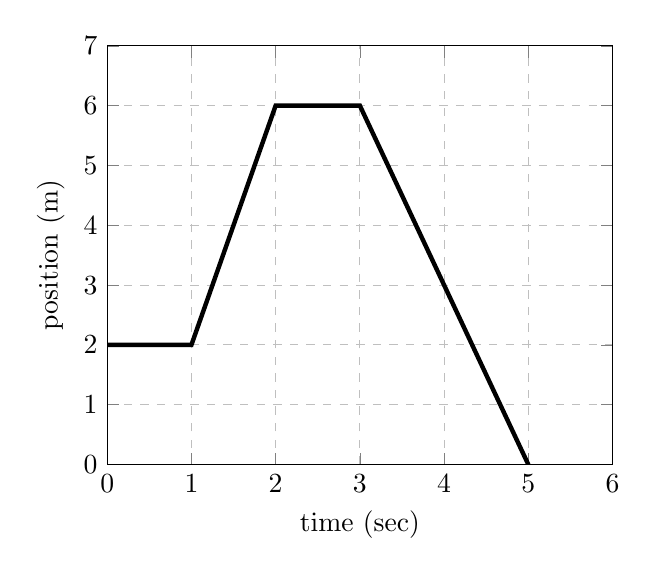
\begin{tikzpicture}
        \begin{axis}[
            xmin=0, xmax=6,
            ymin=0, ymax=7,
            width=8cm,
            ylabel = {position (m)},
            xlabel={time (sec)},
        ]
          \addplot [ultra thick] table {
            x   y
            0   2
            1   2
            2   6
            3   6
            5   0
          };
        \end{axis}
      \end{tikzpicture}
  \end{EnvUplevel}

  \question 
    What is the cat's {\bf position} at 1 second?
    \vs

  \question 
    What is the cat's {\bf position} at 1.5 seconds?
    \vs

  \question 
    What is the cat's {\bf velocity} between 2 and 3 seconds?
    \vs
    
  \question 
    What is the cat's {\bf velocity} between 1 and 2 seconds?
    \vs

  \question 
    What is the cat's {\bf velocity} between 3 and 5 seconds?
    \vs
  
  \pagebreak

  \begin{EnvUplevel}

    Consider the motion of these two cars to answer the following questions.
    
    \begin{multicols}{2}

      \begin{center}
        
        {\bf Car \#1}

        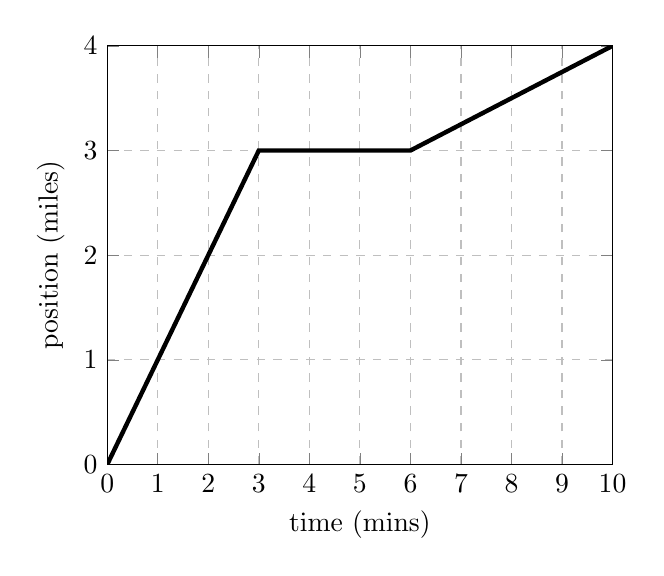
\begin{tikzpicture}
          \begin{axis}[
              xmin=0, xmax=10,
              ymin=0, ymax=4,
              width=8cm,
              ylabel = {position (miles)},
              xlabel={time (mins)},
          ]
            \addplot [ultra thick] table {
              x   y
              0   0
              3   3
              6   3
              10  4
            };
          \end{axis}
        \end{tikzpicture}

        {\bf Car \#2}

        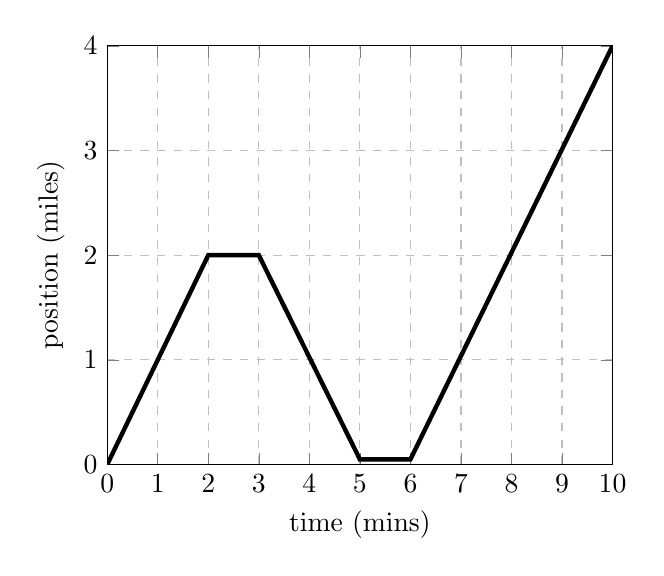
\begin{tikzpicture}
          \begin{axis}[
              xmin=0, xmax=10,
              ymin=0, ymax=4,
              width=8cm,
              ylabel = {position (miles)},
              xlabel={time (mins)},
          ]
            \addplot [ultra thick] table {
              x   y
              0   0
              2   2
              3   2
              5   0.05
              6   0.05
              10  4
            };
          \end{axis}
        \end{tikzpicture}
      
      \end{center}

    \end{multicols}
  \end{EnvUplevel}

  \question
    Which car started out moving faster?  How do you know?
    \vs

  \question
    What was the total time that each car was stopped?
    \vs

  \question 
    Match each of the following statements to the correct segment on one of the graphs.  Write the appropriate letter next to its matching segment on the graph.

    \begin{parts}
      \part Car takes 2 minutes to return home
      \part Car travels 4 miles in 4 minutes
      \part 
        Car stops for 3 minutes while picking up a friend.
      \part Car travels 3 miles toward school in 3 minutes.
      \part 
        The driver, realizing he may have forgotten his homework, pulls over and looks through his backpack for one minute.
      \part 
        Due to traffic, the car moves slowly and only travels one mile in 2 minutes.
      \part Car stops for 2 minutes
    \end{parts}
    
  
  \pagebreak

  \question

    Now, you will be asked to draw your own position vs. tiume graph and come up with a story to describe it just like in the previous problem.

    You must have at least {\bf 5 parts of your story}:  One part must be when you are {\bf stopped}.  One part must be where you are {\bf moving backward}.  The other three are up to you.  For each part, you must include the f distance you wnet and the time that went by.  For example, \emph{``I drove my car for 5 miles in 8 minutes''}.

    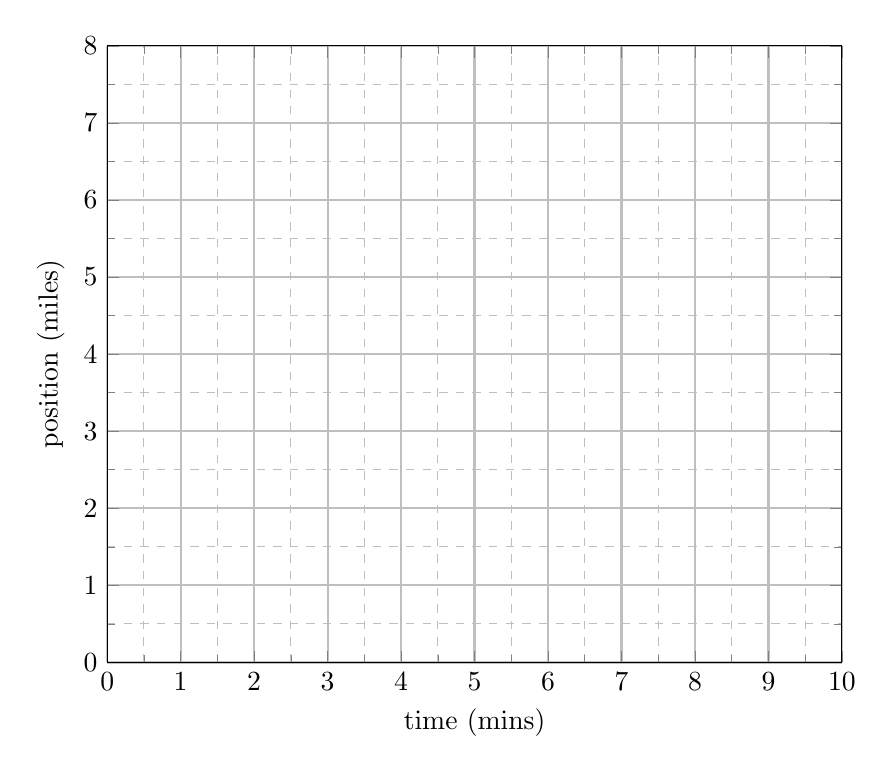
\begin{tikzpicture}
      \begin{axis}[
          xmin=0, xmax=10,
          ymin=0, ymax=8,
          width=.9\textwidth,
          ylabel = {position (miles)},
          xlabel={time (mins)},
          minor tick num = 1,
          grid=both,
          major grid style = {thick, solid},
          minor grid style = dashed,
      ]
      \end{axis}
    \end{tikzpicture}

    Explain what your object is doing here:

\end{questions}
\end{document}